\cleardoublepage
\chapter{Results}
\label{ch:results}

This chapter aims at presenting and discussing the achieved results on the imageclef challenge. Firstly, in section \ref{sec:first} a few examples of some tests that showcase the fine-tuning of the system is presented. Secondly, in section \ref{sec:example} an example on how the system performed in a given topic is showcased and some insight is given on the differences in performance between the submitted runs. Finally, in section \ref{sec:perfomance_results} the achieved results on the challenge are presented.

\section{System Fine-Tuning Using The Dev Topics}
\label{sec:first}

The first tests using the system architecture described on the previous chapter were run on a laptop. The dataset of pictures used was smaller (20.000 images) and not all topics were fully analysed. This tests took between 8h-10h each and they were done in order to find a good weight distribution between each category, detect bugs on the code and overall fine-tune the system before sending the code to the main processing computer (where the fully processing of the dataset took up to 1-2 days).

\begin{figure}[H]
  \centering
  \captionsetup{justification=centering}

  \begin{subfigure}{0.22\textwidth}
  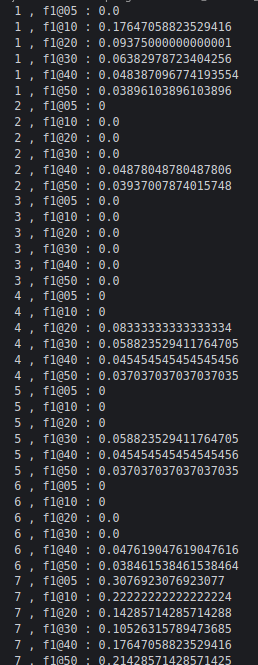
\includegraphics[width=\textwidth]{Sections/7Results/images/runexample5.png} 

  \end{subfigure}
  \begin{subfigure}{0.22\textwidth}
  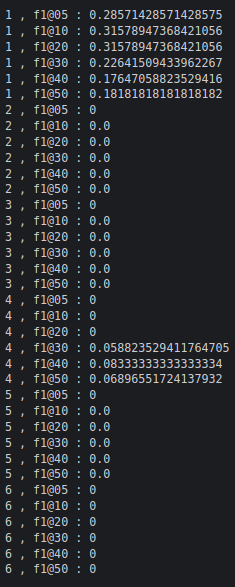
\includegraphics[width=\textwidth]{Sections/7Results/images/runexample3.png}\hfill
  \end{subfigure}
  \begin{subfigure}{0.22\textwidth}
  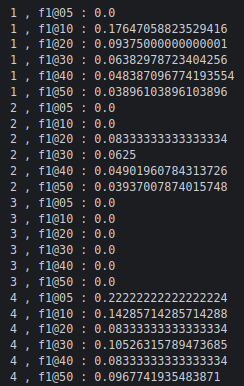
\includegraphics[width=\textwidth]{Sections/7Results/images/runexample4.png}\hfill
  \end{subfigure}
  \caption{Examples of some different results with the fine-tuning of the weight distribution.}
\end{figure}
\newpage

This examples show the performance achieved of the system on a F1-measure@XX measure. The differences in performance on the given examples happen because of the difference in calculations of weights for each category. 


\section{System Performance Example}
\label{sec:example}

This section provides an insight on how the system performed in the imageclef challenge using topic 9 as an example : \\

\textbf{Title}: "Eating pizza".

\textbf{Description}: "Find the moments when u1 was eating a pizza
while talking to one man".

\textbf{Narrative}:" To be considered relevant, the u1 must eat or
hold a pizza with a man visible in the background. The moments that
u1 was talking to more than one person are not relevant".


\subsection{Run 1 and Run 2 Image Retrieval Example}

The following images showcase an excerpt of the csv files generated by both runs that were sent to the imageClef evaluation platform.

The file is organized in the following way: [topic id number, image name, confidence score].


\begin{figure}[H]
  \centering
  \captionsetup{justification=centering}

  \begin{subfigure}{0.4\textwidth}
  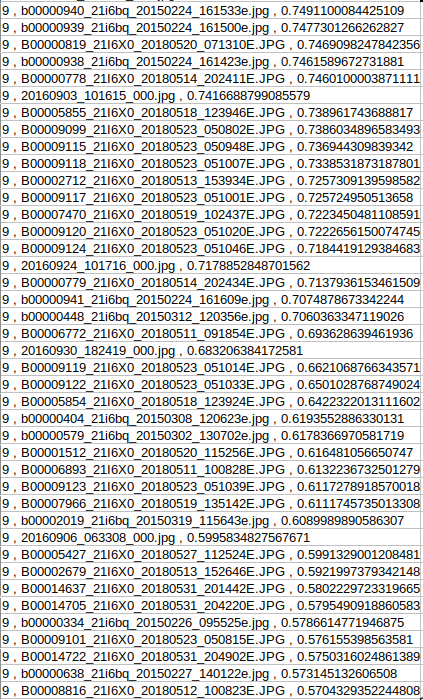
\includegraphics[width=\textwidth]{Sections/7Results/images/topic9_results.png} 
  \caption{Run 1}
  \end{subfigure}
  \hspace{+5mm}
  \begin{subfigure}{0.385\textwidth}
  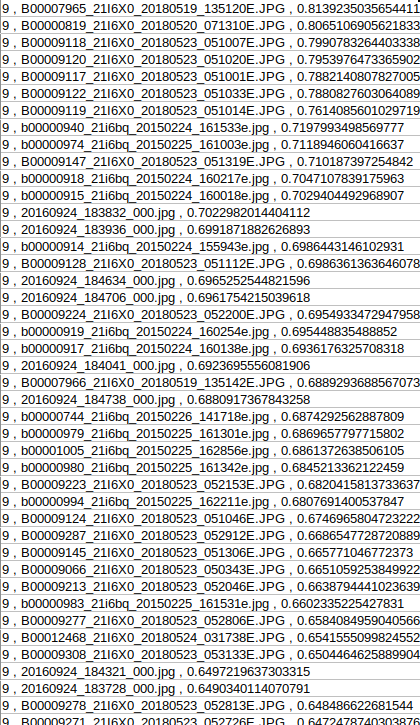
\includegraphics[width=\textwidth]{Sections/7Results/images/topic9results2.png}
  \caption{Run 2}
  \end{subfigure}
  \caption{Achieved results on topic 9 of the test topics.}
  \label{fig:runs_csv}
\end{figure}
\newpage
\subsection{Top 3 Retrieved Image on Run 1}
\label{sec:run1}

As it can be observed in figure \ref{fig:runs_csv} a), the top 3 images that were retrieved for topic 9 in run 1 were:
\begin{enumerate}
  \itemsep0em
  \item b00000940\_21i6bq\_20150224\_161533e.jpg;
  \item b00000939\_21i6bq\_20150224\_161500e.jpg;
  \item B00000819\_21I6X0\_20180520\_071310E.JPG.
\end{enumerate}
 
The images can be seen below.

\begin{figure}[H]
  \centering
  \captionsetup{justification=centering}

  \begin{subfigure}{0.32\textwidth}
  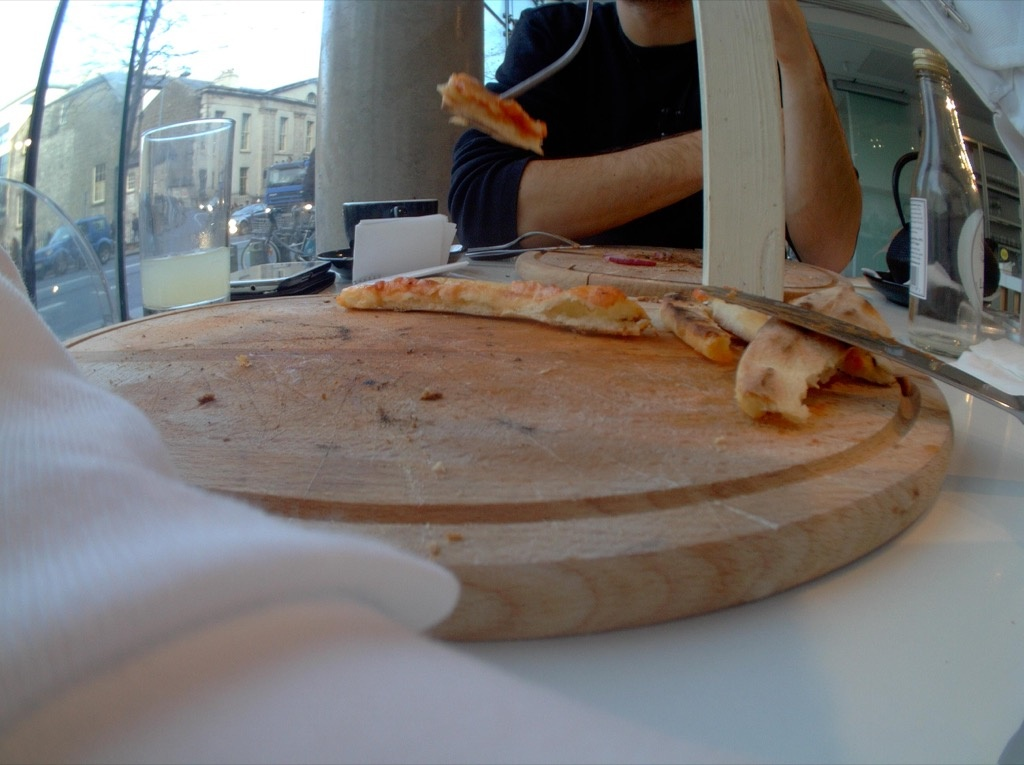
\includegraphics[width=\textwidth]{Sections/7Results/images/top1.jpg} 
  \caption{Top 1}

  \end{subfigure}
  \begin{subfigure}{0.32\textwidth}
  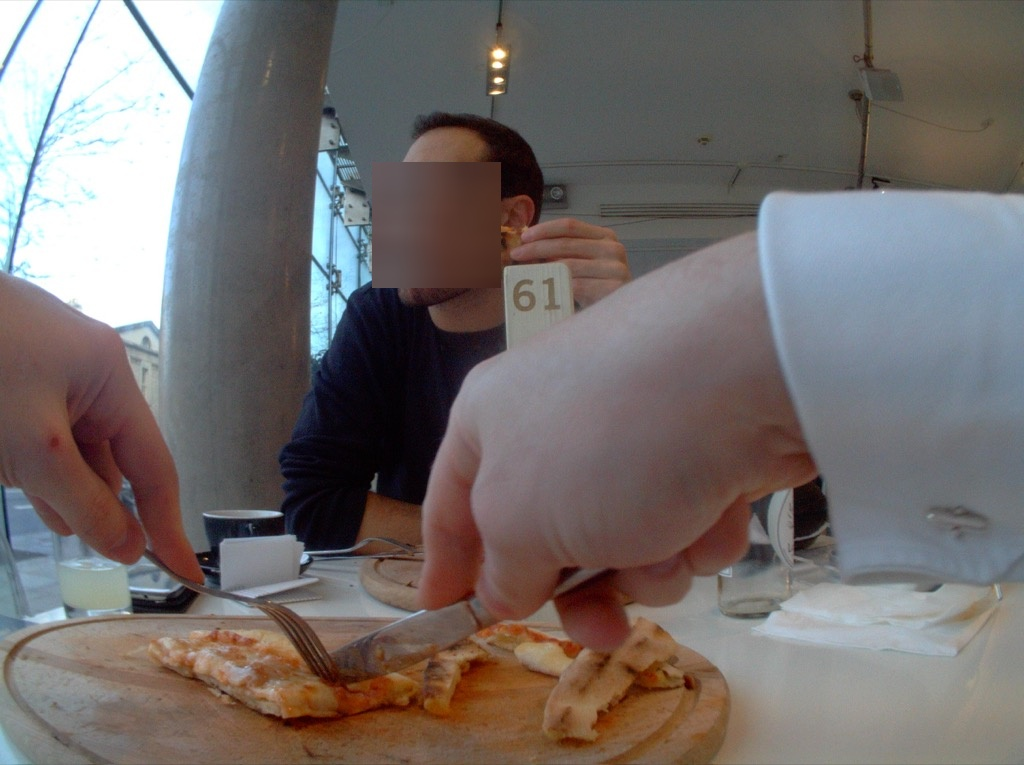
\includegraphics[width=\textwidth]{Sections/7Results/images/top2.jpg}\hfill
  \caption{Top 2}
  \end{subfigure}
  \begin{subfigure}{0.32\textwidth}
  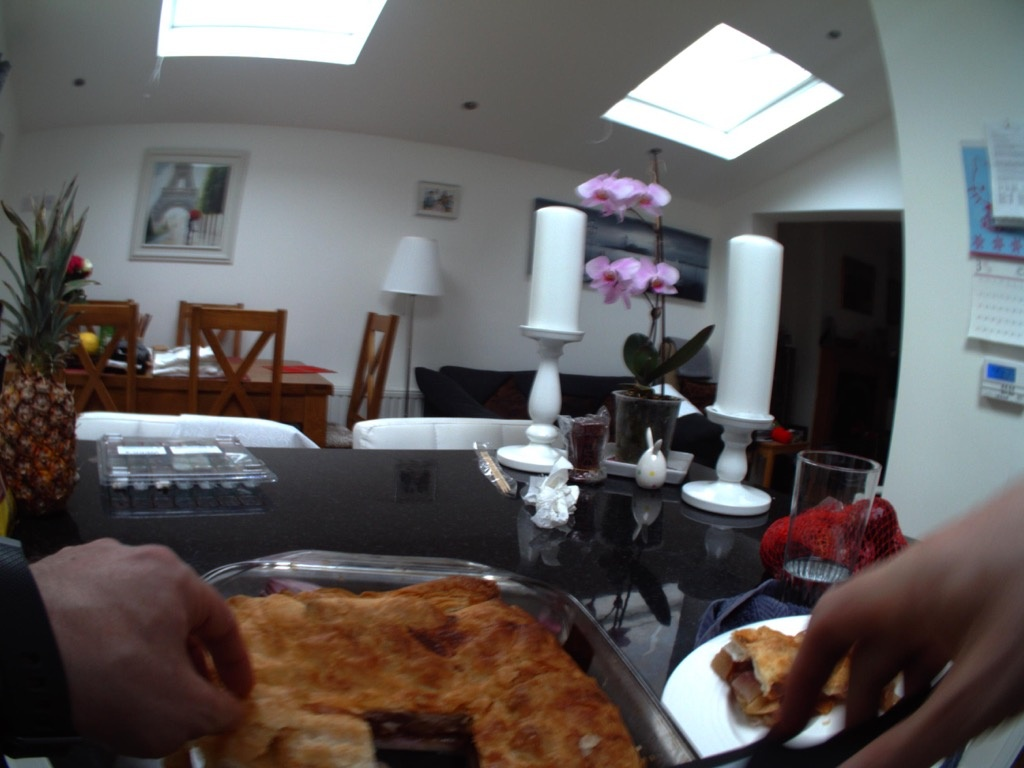
\includegraphics[width=\textwidth]{Sections/7Results/images/top3.jpg}\hfill
    \caption{Top 3}
  \end{subfigure}
  \caption{Top 3 retrieved pictures for topic 9 on run 1}
\end{figure}


\subsection{Top 3 Retrieved Images on Run 2}

Using again figure \ref{fig:runs_csv}, the top 3 images that were retrieved for topic 9 on run 2 were: 


\begin{enumerate}
  \itemsep0em
  \item B00007965\_21I6X0\_20180519\_135120E.JPG;
  \item B00000819\_21I6X0\_20180520\_071310E.JPG;
  \item B00009118\_21I6X0\_20180523\_051007E.JPG.
\end{enumerate}


The images can be seen below.
\begin{figure}[H]
    \centering
    \captionsetup{justification=centering}
  
    \begin{subfigure}{0.32\textwidth}
    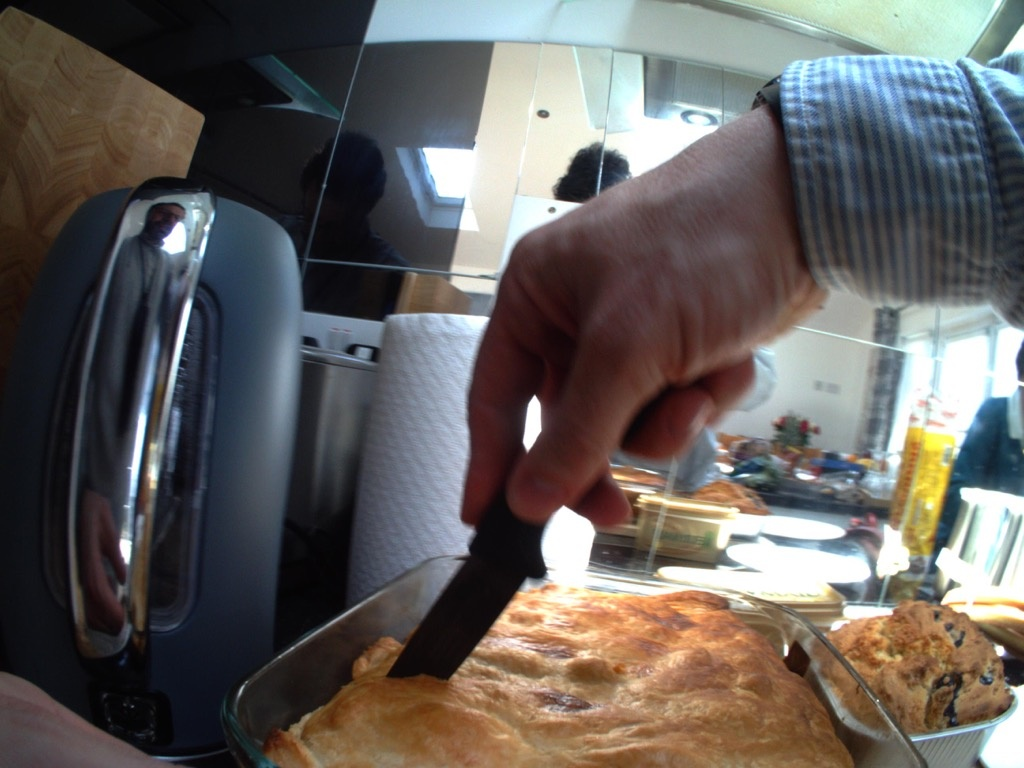
\includegraphics[width=\textwidth]{Sections/7Results/images/run2top1.jpg} 
    \caption{Top 1}
  
    \end{subfigure}
    \begin{subfigure}{0.32\textwidth}
    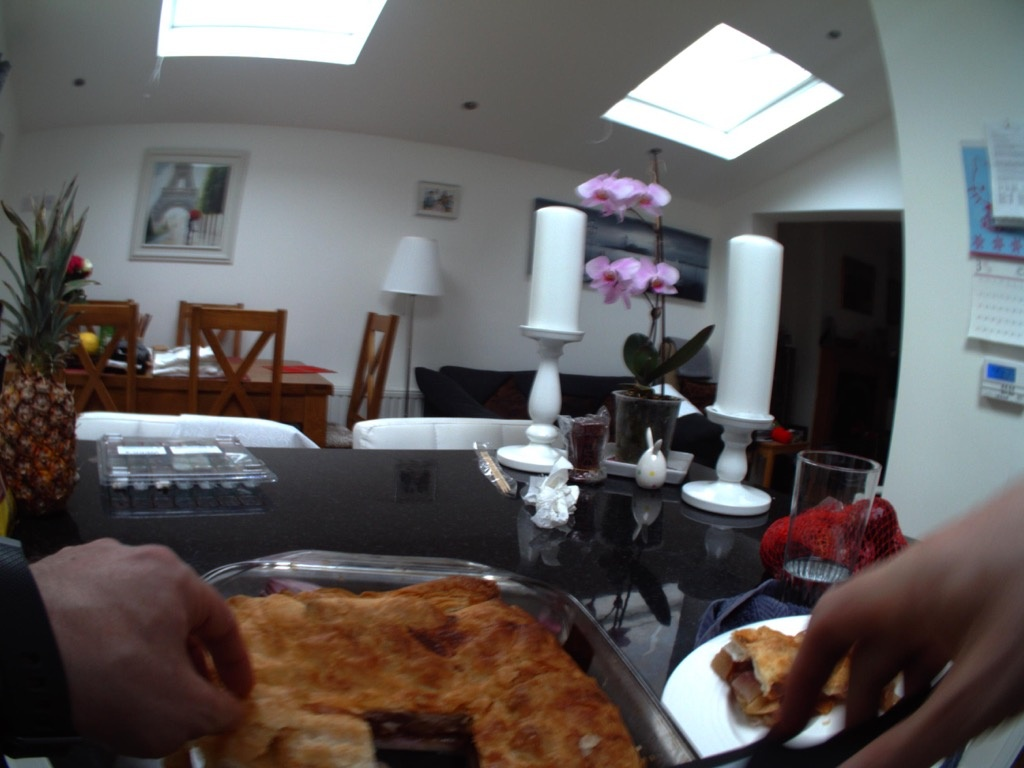
\includegraphics[width=\textwidth]{Sections/7Results/images/run3top2.jpg}\hfill
    \caption{Top 2}
    \end{subfigure}
    \begin{subfigure}{0.32\textwidth}
    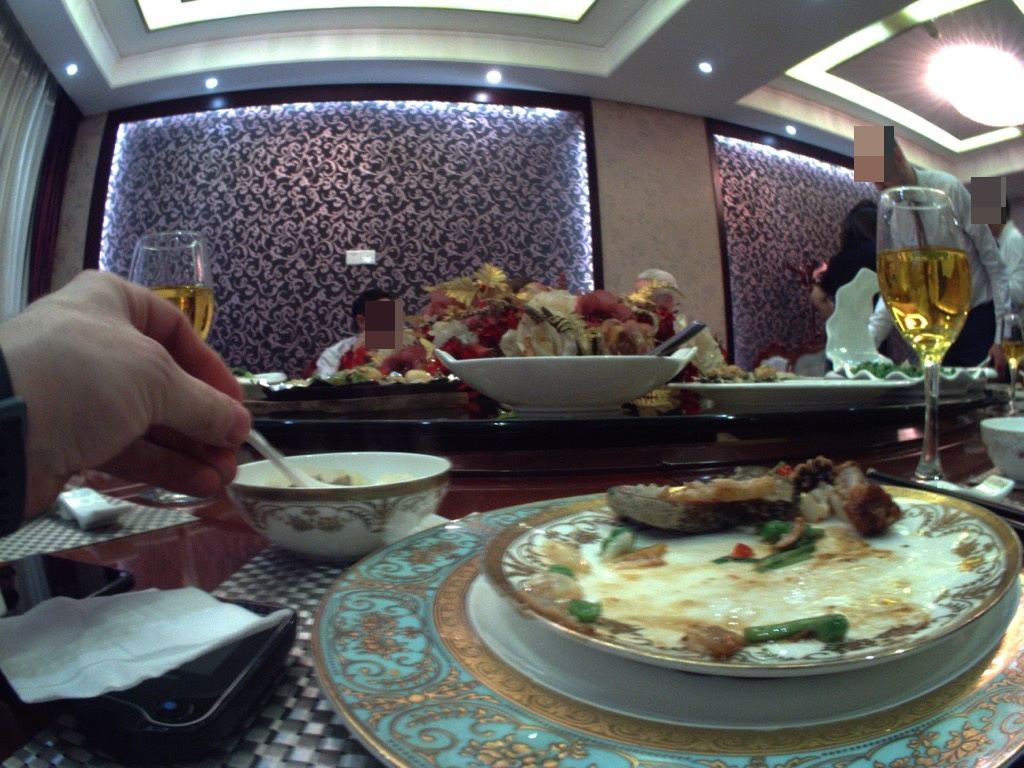
\includegraphics[width=\textwidth]{Sections/7Results/images/run2top3.jpg}\hfill
      \caption{Top 3}
    \end{subfigure}
    \caption{Top 3 retrieved pictures for topic 9 on run 2}
  \end{figure}

  \newpage

  \subsection{Topic 9 Performance Analysis}

  Even if the top 10 pictures are the ones that count for the performance evaluation of the run, the top 3 pictures are already representative the system efficiency. It is clear that for topic 9 the run 1 achieved better performance, since the first 2 pictures clearly belong to the moment described in topic 9. The third picture however does not belong to topic 9 since it is a picture of a person eating a lasagne alone but it is a similar scenario.
  
  Run 2 however did not retrieved any single picture from topic 9 on the top 3 pictures, however the scenario is identical. All of the 3 photos are representative of food being eaten. However, something to note is that run 2 confidence scores are higher than run 1, but run 1 achieved better practical results. Some possible reasons for this to occur may be :

  \begin{itemize}
    \itemsep0em
    \item The negative categories on run 1 might have decreased the confidence score on  pictures that don't belong to the topic.
    \item The object detection algorithm on run 1 providing better detections than the algorithm used for run 2.
    \item The category weight distribution on run 2 decreasing the weight on some categories that were important for the confidence score calculation in the images that belong to the topic.
    \item The difference in the similarity score between the different visual concepts on each run might also impact the performance of the system.
  \end{itemize}



\section{Achieved Overall Performance Results}
\label{sec:perfomance_results}

Table \ref{table:2019} and table \ref{table:2020} provides an overview of the achieved performance results in different runs for different systems that were obtained in the year 2019 and 2020 for the ImageCLEFlifelog LMRT subtask. 
\newcolumntype{P}[1]{>{\centering\arraybackslash}p{#1}}
\begin{table}[H]
    
    \centering
\begin{tabular}{ |P{4cm}|P{2.5cm}|P{2cm}|P{3cm}|  }
    \hline
    \multicolumn{4}{|c|}{\textbf{2019 Results}} \\
    \hline
    Team & System Type & Run Name & F1-measure@10 \\
    \hline
    UA.PT Bioinformatics  & automatic  & Run 1   &  0.016 \\
    UA.PT Bioinformatics  & automatic  & Run 2   &  0.026 \\
    UA.PT Bioinformatics  & automatic  & Run 3   &  0.027 \\
    UA.PT Bioinformatics  & automatic  & Run 4   &  0.027 \\
    UA.PT Bioinformatics  & automatic  & Run 5   &  0.036 \\
    UA.PT Bioinformatics  & automatic  & Run 6   &  0.057 \\
    \hline
    \multicolumn{4}{|c|}{\textbf{Best Results Achieved by a Team}} \\
    \hline
    HCMUS  & interactive  & Run 2   &  0.61 \\
    \hline        
    \end{tabular}
    \caption{Results obtained in 2019 from UA.PT Bioinformatics \cite{Ribeiro2019} and the best team \cite{Le2019}. }
    \label{table:2019}
\end{table}
\begin{table}[H]
    \centering
\begin{tabular}{ |P{4cm}|P{2.5cm}|P{2cm}|P{3cm}|  }   
    \hline
    \multicolumn{4}{|c|}{\textbf{2020 Results}} \\
    \hline
    Team & System Type & Run Name & F1-measure@10 \\
    \hline
    UA.PT Bioinformatics  & automatic  & Run 1   &  0.03 \\
    UA.PT Bioinformatics  & automatic  & Run 2   &  0.03 \\
    UA.PT Bioinformatics  & interactive  & Run 3  &  0.54 \\
    \hline
    \multicolumn{4}{|c|}{\textbf{Best Results Achieved by a Team}} \\
    \hline
    HCMUS  & interactive  & Run 10   &  0.81\\
    \hline       
    \end{tabular}
    \caption{Results obtained in 2020 from UA.PT Bioinformatics \cite{Ribeiro2020} and the best team \cite{Ninh2020}.}
    \label{table:2020}
\end{table}

\subsection{Overall Performance Analysis}

Comparing the table \ref{table:2019} that shows the results of the year 2019 and table \ref{table:2020} that shows the results of this year challenge, it is clear that there was no overall improvement on an automatic system performance. Furthermore, it is also possible to clearly see the difference in performance between interactive systems and fully automatic systems. Having user interaction and visualizations yields much better results than having a fully automatic system.

The tables shown make a strong argument that for the imageclef LMRT sub-task an interactive approach is a much better suited method, the user visualization and interaction with the application allows for much more accurate results since the user can chose the picture that he thinks are correct for the corresponding moment.

Another important aspect to notice is that the results of the automatic approach this year achieved the same exact F1-measure@10 score, this is highly do to the fact that even when using different state-of-the-art object detection algorithms, different weights for each category and even using negative categories on one run and not on the other, much of the data used for both runs was provided by the organizers which is a highly faulty and inaccurate.



